\section{Формулы}

\subsection{Аналитический функтор для h-species}

\tikzset{node distance=2cm, auto}
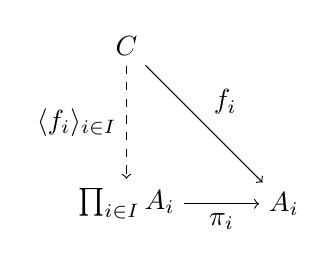
\begin{tikzpicture}
  \node (C) {$C$};
  \node (P) [below of=C] {$\prod_{i \in I} A_i$};
  \node (Ai) [right of=P] {$A_i$};
  \draw[->] (C) to node {$f_i$} (Ai);
  \draw[->, dashed] (C) to node [swap] {$\langle f_i \rangle_{i \in I}$} (P);
  \draw[->] (P) to node [swap] {$\pi_i$} (Ai);
\end{tikzpicture}

\subsection{Фробениусова характеристика}

В этом разделе мы напишем формулу для Фробениусовой характеристики.
То есть подчитаем количество неподвижных раскрасок.

Напомним, что в случае обычных species формула выглядит так:
\begin{equation}
\label{eq:fr}
\sum_{\lambda \vdash n}\chi(\sigma_{\lambda}) \frac{\phi^{\lambda}}{z_{\lambda}}
\end{equation}

Где $\chi$ --- характер (перестановочного) представления, $\sigma$ ---
перестановка цикленного типа $\lambda$, 
$\phi^{\lambda} = 
(x_1^{\lambda_1} + x_2^{\lambda_1} + x_3^{\lambda_1} + \dots)
(x_1^{\lambda_2} + x_2^{\lambda_2} + x_3^{\lambda_2} + \dots)
(x_1^{\lambda_3} + x_2^{\lambda_3} + x_3^{\lambda_3} + \dots)
\dots$,
 $z_\lambda$ --- индекс класса сопряженности $\sigma$.
Появляется она из следующих соображений: в числителе стоит симметрическая
функция считающая все неподвижные раскраски. Цвета это $x_1, x_2, x_3, \dots$

Формула для h-species будет следующей
\begin{equation}
\label{eq:h-fr}
\sum_{\lambda^1 + \lambda^2 \vdash n}\chi(\sigma_{\lambda^1 \lambda^2})
\frac{\Bar{\phi}^{\lambda^1} \phi^{\lambda^2}}{z_{\lambda^1 \lambda^2}}
\end{equation}

Циклы в каждом элементе $H_n$ бывают двух типов:
длинные --- каждая грань входит в цикл вместе со своей противоположной гранью и
короткие --- пара граней лежит в симметричных, различных циклах. Здесь
$\lambda^1$ --- цикленный тип коротких перестановок, $\lambda^1$ --- цикленный тип длинных перестановок.
В пояснении нуждается числитель. Дело в том что длинный цикл соответсвует
одному цвету, а пара симметричных коротких может быть либо покрашена в один
цвет, либо в два оттенка одного цвета (???что-то тут не то???).
